\chapter{Atomkerne und Kernmodelle}
\begin{itemize}
\item[$\ra$] Geometrie von Kernen
\item[$\ra$] Kernzusammensetzung
\item[$\ra$] Modelle für Kernmassen etc.
\end{itemize}

\section{Kernradien und Formfaktor}
\begin{itemize}
\item Experimentelle Untersuchung der Kerngrößen durch Streuexperimente
\begin{align}
\begin{matrix}
(e^- , \alpha) & A & \ra & (e^- , \alpha)\ A & \text{(el. Ladung)}\\
\underbrace{\ n \ } & \underbrace{\ A \ } & \underbrace{\ \ra \ } & n\ A & \text{(Massendichte)} \\
 \text{\glqq Sonde\grqq} & \text{Kern} & \text{el. Streuung} & & 
\end{matrix}
\end{align}
Typische Energien: $E_\mr{kin}\sim 1 \text{ bis } 100\,\mr{MeV}$\\
Gute Näherung: $E_\mr{kin} \ll M_A$\\
$\Rightarrow$ Energieübertrag auf Kern ist vernachlässigbar
\begin{figure}[!ht]
	\centering
	\begin{tikzpicture}
	\begin{feynman}
	\vertex (a1);
	\node[right = 3cm of a1, blob] (a2) {A};
	\vertex[above right = 3cm of a2] (c1);
	\vertex[below right = 3cm of a2] (d1);
	
	\diagram*{
	(a1) -- [fermion, edge label = {$e$,$\alpha$,$\vec p$}] (a2),
	(a2) -- [fermion, edge label = {$e$,$\alpha$,$\vec p^{\;\prime}$}] (c1),
	(a2) -- [fermion] (d1)
	};
	\end{feynman}
	\end{tikzpicture}
	\caption{Energieübertrag auf Kern durch Stoß\label{fig:4.1}}
\end{figure}
\begin{align}
E^A_\mr{kin}=\frac{q^2}{2M_A} \ll \frac{p^2}{2m_{\alpha,e}}=E^{\alpha,e}_\mr{kin}
\end{align}
(Achtung: für $\alpha$-Streuung an leichten Kernen nicht gültig, da $\labs\vec{p}\rabs = \labs \vec{p}^\prime\rabs$)\\
\begin{figure}[!ht]
	\centering
	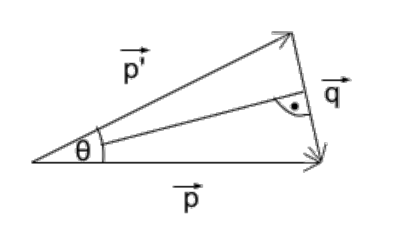
\includegraphics[width=.35\textwidth]{imgs/ep5-fig-4-2.pdf}
	\caption{Impulsübertrag $q$ eines elastisch gestreuten Teilchens \label{fig:4.2}}
	\end{figure}
Aus Abb. \ref{fig:4.2} ergibt sich für $q^2= (\vec p - \vec{p}^\prime)^2$:
\begin{align}
q^2=\lb 2\labs \vec{p}\rabs \sin\frac{\theta}{2}\rb ^2 = \lb  2 p \sin \frac{\theta}{2}\rb ^2
\end{align}
\begin{figure}[!ht]
	\centering
	\begin{tikzpicture}
    \begin{feynman}
    \vertex (a1);
    \vertex [below right= 3cm of a1] (a2);
    \vertex [above right= 3cm of a2] (a3);
    \node [below= of a2, blob] (b2);
    
    \diagram*{
    (a1) -- [fermion, edge label = $e^-$] (a2),
    (a2) -- [fermion, edge label = $e^-$] (a3),
    (a2) -- [photon, edge label = $\gamma$] (b2),
    };
    \end{feynman}
    \end{tikzpicture}
	\caption{Feynman-Diagramm der elektromagnetischen Wechselwirkung mit dem Kern $A$\label{fig:4.3}}
	\end{figure}
    
$\Rightarrow$ der WQ ist elm. (vgl.Abb.\ref{fig:4.3}), daher Coulomb-Streuung
\begin{align}
\begin{split}
\frac{\Pa \sigma}{\Pa \Omega}\sim (e^2)(Ze^2)\frac{1}{q^4}\sim Z^2\alpha^2\frac{1}{q^4}\\
q^2 \text{ in } q^4 \text{ gegeben durch } q^2=\underbrace{\lb E-E^\prime \rb ^2}_{=0}-\vec{q}^2\\
\Rightarrow q^2=-4p^2\sin^2\frac{\theta}{2}\\
\Rightarrow \boxed{\frac{d\sigma}{d\Omega}\sim \frac{Z^2\alpha^2}{16p^4 \sin^4 \frac{\theta}{2}}}\\
\sim\text{ Rutherford-WQ}
\end{split}
\end{align}
\begin{itemize}
\item[$\ra$] starke $p$- und $\theta$-Abhängigkeit
\item[$\ra$]  maximales $\labs \vec{q} \rabs$ für $\theta=180^{\circ}$
\begin{itemize}
\item[$\ra$]  stärkste Annäherung
\item[$\ra$]  kleinster WQ
\end{itemize}
\item[$\ra$]  $e^-$ relativistisch
\item[$\ra$]  $\alpha$ nicht-relativistisch
\end{itemize}

\item Was ändert sich, wenn A ausgedehnte Ladungsverteilung $\rho\lb \vec{r}\rb $ hat?
\begin{align}
\left. \frac{\Pa \sigma}{\Pa \Omega}\right|_\mr{Coul}\rightarrow \left. \frac{\Pa \sigma}{\Pa \Omega}\right|_\mr{Coul}\cdot \left|F\lb \vec{q}\rb \right|^2
\end{align}

Hierbei ist der Formfaktor $F\lb \vec{q}\rb $ eingeführt worden. Er errechnet sich als Fouriertransformierte der Ladungsverteilung.
\begin{align}
\boxed{F\lb \vec{q}\rb =\frac{1}{Ze}\int e^{i\vec{q}\vec{r}}\rho \lb \vec{r}\rb  \Pa^3 r}
\end{align}
(Offenbar gleich zu Beugungseffekt: QM Störungsrechnung (mehr in Kap. 6))
\begin{itemize}
\item Messung von $\frac{\Pa \sigma}{\Pa \Omega}$
\item[$\ra$] Bestimmung von $\labs F\lb \vec{q}\rb  \rabs ^2$
\item[$\ra$] Bestimmung von $\rho(\vec{r})$
\end{itemize}

Ergebnis für $\rho(\vec{r})=\rho\lb r\rb $ bei homogener Ladungsverteilung (Abb. \ref{fig:4.4}):
\begin{align}
\boxed{\rho\lb r\rb =\frac{\rho_0}{1+e^{\frac{r-a}{b}}}}
\end{align}
Typische Werte der Parameter $a$, $b$:
\begin{align}
\boxed{a=1.07 \mr{A^{\nicefrac{1}{3}}\,fm} \qquad b=0.54\,\mr{fm}}
\end{align}
Gleiches $\rho_0$ homogener Ladungsverteilung, scharfer Rand:
\begin{align*}
\boxed{R_A=1.21 A^{\nicefrac{1}{3}}\,\mr{fm}}
\end{align*}
\end{itemize}
\begin{figure}[!ht]
	\centering
	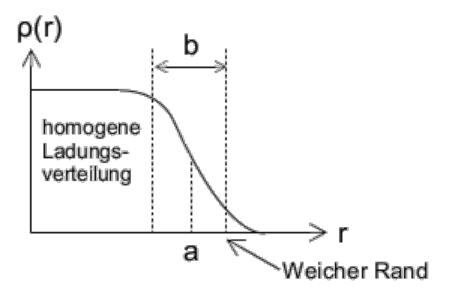
\includegraphics[width=.35\textwidth]{imgs/ep5-fig-4-4.pdf}
	\caption{Homogene Ladungsverteilung in einem Teilchen/Kern\label{fig:4.4}}
	\end{figure}

\section{Kernaufbau und Bindungsenergie}
Ein Atomkern besteht aus
\begin{align*}
\boxed{ \begin{matrix}
Z & \text{Protonen (p)}\\ N & \text{Neutronen (n)}\\ Z + N = A & \text{Nukleonen (p+n)}
\end{matrix} \ A: \ \text{Massenzahl} }
\end{align*}
Schreibweise: $^A_Z X_N$ mit $X$ als Elementsymbol\\
z.B. $^{12}_6 C_6$, auch $^{12}_6 C$, $^{12}C\ \lsb C12,12C\rsb $ \\
\begin{figure}[!ht]
	\centering
	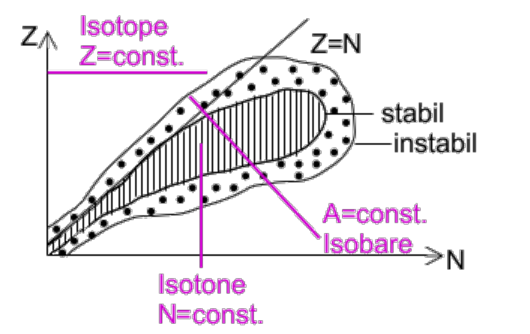
\includegraphics[width=.5\textwidth]{imgs/ep5-fig-4-5.pdf}
	\caption{Nuklidkartenskizze in der N-Z-Ebene \label{fig:4.5}}
	\end{figure}

\begin{itemize}
\item[$\ra$] \textbf{Bindungsenergie}\\
Energie $\mathcal{O}(10\,MeV)$ nötig, um Nukleonen aus Kern zu lösen.\\
Gesamte Bindungsenergie eines Atoms:
\begin{align}
E_B(A,Z)=\underbrace{E(Zp+Nn+Ze^-)}_{ZM_p+NM_n+Zm_e}-\underbrace{E(^A_Z X_N)}_{M(^A_Z X_N)=M(A,Z)}
\end{align}
Oft:
\begin{align}
\boxed{\Delta M=-E_B \,\widehat{=}\, \text{Massendefekt}}
\end{align}
Messung von $E_B$ erfordert präzise Messung von Atom/Kernmassen
\begin{itemize}
\item[$\Ra$] Massenspektroskopie (Ablenkung in $E$- und $B$-Feldern, $\frac{\Delta M}{M}\sim \mathcal{O}(10^{-6})$)
\item[$\Ra$] Ergebnis: $E_B \simeq 1\%$ von $M(A,Z)$
\item[$\lt$] viel größer als bei elm. WW ($10^{-6}$ bis $10^{-8}$ bei Atomen)
\end{itemize}
\begin{figure}[!ht]
	\centering
	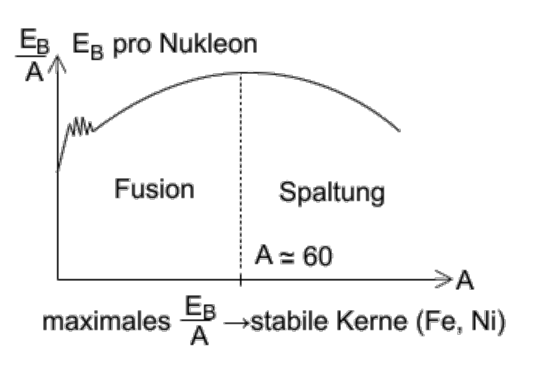
\includegraphics[width=.5\textwidth]{imgs/ep5-fig-4-6.pdf}
	\caption{Bindungsenergie pro Nukleon über die Nukleoenenzahl aufgetragen. Erkennbar ein Maximum, zu welchem Kerne fusioniert werden können zur Energiegewinnung und oberhalb dessen Kerne gespalten werden \label{fig:4.6}}
	\end{figure}
\begin{itemize}
\item[$\ra$] stabile Kerne mit $A\leq 60$:\\
Energiegewinn durch Fusion (Sonne!)
\item[$\ra$] stabile Kerne mit $A>60$:\\
Energiegewinn durch Spaltung (Kernkraftwerke, -waffen)
\end{itemize}
Können wir $\frac{E_B}{A}$ verstehen?
\begin{itemize}
\item[$\ra$] wenn starke WW langreichweitig (wie Coulomb)\\
$E_B\sim \frac{1}{2}A(A-1)\leftarrow$ Zahl der Nukleonenpaare\\
Aber: $E_B\sim A$
\item[$\Ra$] $\boxed{\text{starke WW kurzreichweitig (Nukleon \glqq sieht\grqq nur nächste Nachbarn)}}$
\end{itemize}
\end{itemize}

\section{Tröpfchenmodell und Weizsäcker-Massenformel}
Das sogenannte Tröpfchenmodell war das erste Modell der Kernphysik zur Beschreibung deren Eigenschaften. Da es das erste ist, ist es auch durchaus inkomplett.\footnote{Der Physiker Weizsäcker ist der Bruder des ehemaligen Bundespräsidenten}

\begin{itemize}
\item[$\rightarrow$] Kerndichte $\approx \ const.$
\item[$\rightarrow$] Kerne sphärisch
\item[$\rightarrow$] \glqq Verdampfungsenergie\grqq{} $\sim \ M$
\item[$\Rightarrow$] Wie bei (Wasser)tröpfchen!
\end{itemize}
Modell aus 1930er Jahren (formuliert von Weizsäcker, Williams, Gamov, Bohr):
\begin{align}
\boxed{ E_B = a_v A - a_s A^{\nicefrac{2}{3}} - a_c \frac{Z^2}{A^{\nicefrac{1}{3}}} - a_a \frac{(N-Z)^2}{A} - \frac{\delta}{A^{\nicefrac{1}{2}}}}
\end{align}
\begin{compactitem}
\item[mit] $a_vA \ =$ \textbf{Volumenterm}\\
$a_v$ Bindung der Nukleonen an ihre Nachbarn
\item[] $-a_sA^{\nicefrac{2}{3}}\ = $ \textbf{Oberflächenterm}\\
$a_s \approx 18\,$MeV, Nukleonen an der Oberfläche haben weniger Nachbarn, Effekt $\sim R^2 \sim A^{\nicefrac{2}{3}}$ mit $R^3 \sim A$
\item[] $-a_c \frac{Z^2}{A^{\nicefrac{1}{3}}} \ =$ \textbf{Coulombterm}\\
$a_c \approx 0.7\,$MeV, Energie einer homogen geladenen Kugel $\sim \frac{Q^2}{R}$ (Abstoßung der p)
\item[] $-a_a\frac{(N-Z)^2}{A}\ = $ \textbf{Asymmetrieterm}\\
$a_a \approx 23$\,MeV, p, n haben Spin $\nicefrac{1}{2}$ (Fermionen)\\
$\Rightarrow$ Pauli-Prinzip
\item[] $-\frac{\delta}{A^{\nicefrac{1}{2}}} \ =$ \textbf{Paarungsterm},
\begin{align}
\delta = \left\lbrace \begin{matrix} -11\,\mathrm{MeV}& gg\\ 0 & gu,\ ug\\ +11\,\mathrm{MeV} & uu \end{matrix}\right.
\end{align}
$u=$ ungerade, $g=$ gerade, $gg=$ $N$ gerade und $Z$ gerade
\end{compactitem}

\begin{figure}[!ht]
\centering
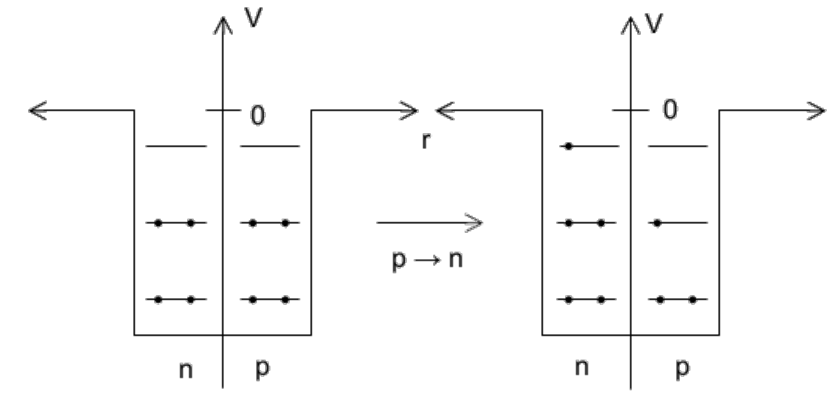
\includegraphics[width=.5\textwidth]{imgs/ep5-fig-4-7.pdf}
\caption{Umwandlung eines Protons in ein Neutron \label{fig:4.7}}
\end{figure}

Gepaarte Nukleonen sind stärker gebunden als \glqq einzelne\grqq{}
\begin{itemize}
\item[$\leadsto$] Modell kann $E_B(A,Z)$ grob beschreiben (insbesondere auch die Region der stabilen Kerne).
\item[$\rightarrow$] Aber:
\begin{compactitem}
\item QM-Effekte \glqq von Hand\grqq
\item Keine Dynamik (Nukleonen im Kern bewegen sich: $\Delta x \cdot \Delta p \gtrsim \hbar$)
\item Keine feineren Strukturen in $E_B(A,Z)$
\item keine Aussagen über Spin, magn. Moment, Parität
\end{compactitem}
\item[$\leadsto$] Interessant: Mit Gravitations- statt Coulombterm $\rightarrow$ Neutronenstern $\approx$ stabile Lösung
\end{itemize}

\section{Das Fermigasmodell}
\begin{figure}[!ht]
\centering
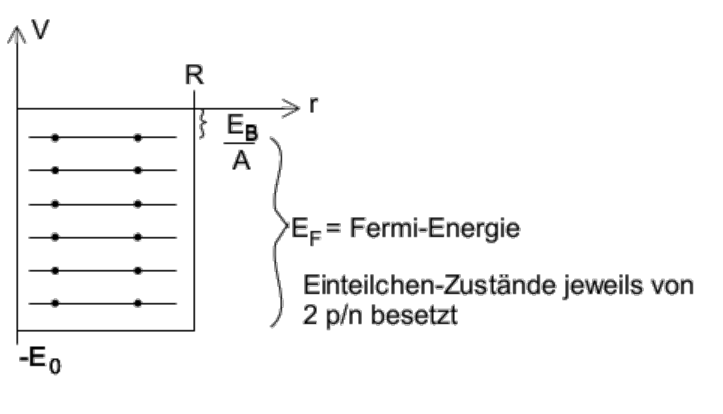
\includegraphics[width=.5\textwidth]{imgs/ep5-fig-4-8.pdf}
\caption{Potentialtopf nach dem Fermigasmodell \label{fig:4.8}}
\end{figure}
Nukleonen gebunden durch WW mit allen anderen Nukleonen.
\begin{itemize}
\item[$\rightarrow$] Effektives Potential
\item[$\rightarrow$] Einfache Näherung: Kastenpotential
\item[$\leadsto$] Wie groß sind $E_F$, $p_F= \sqrt{2M_NE_F}$, $E_0$, $\nicefrac{E_B}{A}$
\item[$\leadsto$] Achtung: $E_0^{(n)} < E_0^{(p)}$ wegen Coulomb-WW der $p$
\begin{compactitem}
\item[$\leadsto$] zunächst vernachlässigt
\end{compactitem}
\end{itemize}
Erinnerung an Quantenmechanik:
\begin{center}
$\boxed{\text{QM: 1 Zustand pro Phasenraumvolumen }(\Delta x\, \Delta p)^3 = \mathrm{h}^3}$
\end{center}
Gesamtes Phasenraumvolumen im Kern:
\begin{align}
\Delta x^3 \rightarrow V_K = \frac{4 \pi}{3} R_n^3\\\Delta p^3 \rightarrow V_p = \frac{4 \pi}{3}p_F^3
\end{align}
\begin{itemize}
\item[$\Rightarrow$] Zahl der Zustände
\begin{align}
\boxed{n= \frac{1}{h^3} \lb  \frac{4\pi}{3} R_n^3\rb \lb \frac{4\pi}{3} p_F^3\rb = \frac{N+Z}{4}= \frac{A}{4}}
\end{align}
\begin{compactitem}
\item[mit] $R_n = R_0 A^{\nicefrac{1}{3}}$, $R_0 = 1.21$\,fm
\end{compactitem}
\begin{align}
\Rightarrow\ \boxed{p_F = \frac{\hbar}{R_0}\lb \frac{9 \pi}{8}\rb ^{\nicefrac{1}{3}} = \frac{197\,\mathrm{MeV\,fm}}{1.21\,\mathrm{fm}}\lb \frac{9 \pi}{8}\rb ^{\nicefrac{1}{3}} = 250\,\mathrm{MeV}}
\end{align}
\item[$\leadsto$] hoher Impuls, etwa wie von Unschärferelation erwartet $\lb \Delta p \sim \frac{\hbar}{R_0}\rb $
\item[$\leadsto$] durch $eA$-Streuung bestätigt
\begin{align}
\lt \ \boxed{{E_F} = \frac{p_F^2}{2M_N} \approx 33\,\mathrm{MeV} \Rightarrow\ E_0 = E_F+ \frac{E_B}{A} \approx 40 \, \mathrm{MeV}}
\end{align}
\item[$\leadsto$] Genauer: mit Coulombpotential
\item[$\leadsto$] Rechnung mit $p_F^{(n)} \neq p_F^{(p)}$ ergibt:
\begin{align}
E_\mathrm{min}^\mathrm{tot} \sim A + \frac{5}{9} \frac{(N-Z)^2}{A}
\end{align}
zweiter Summand erklärt Asymmetrieterm
\item[$\leadsto$] Paarungsterm: Beispiel $^{40}$K, $^{40}$Ca
\end{itemize}

\begin{figure}[!ht]
\centering
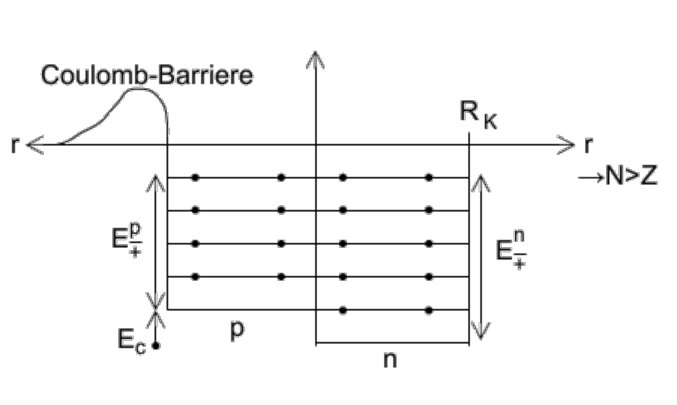
\includegraphics[width=.5\textwidth]{imgs/ep5-fig-4-9.pdf}
\caption{Potentialtopf mit Berücksichtigung der verschiedenen Bindungsenergien für Neutronen und Protonen \label{fig:4.9}}
\end{figure}

\begin{figure}[!ht]
\centering
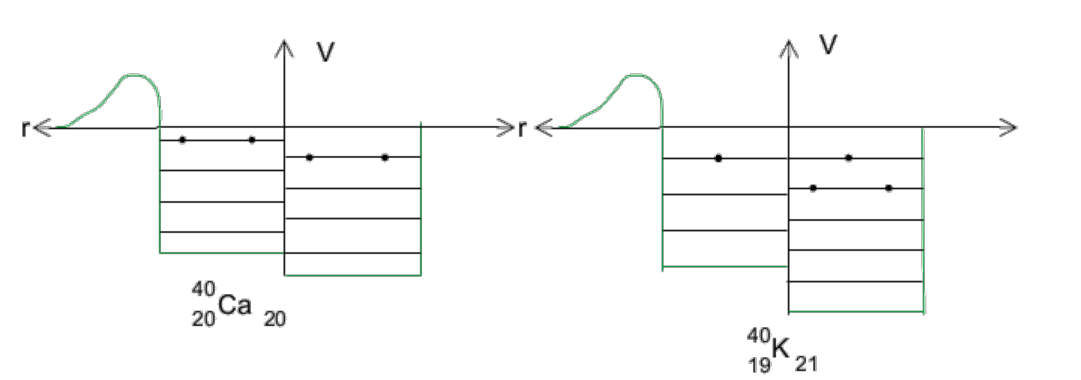
\includegraphics[width=.5\textwidth]{imgs/ep5-fig-4-10.pdf}
\caption{Potentialtopf am Beispiel für Kalium und Calcium \label{fig:4.10}}
\end{figure}

Fermigasmodell:
\begin{compactitem}
\item einfachstes QM-Modell von Kernen
\item erklärt qualitativ QM-Terme in Weizsäcker-Formel
\item aber: keine Vorhersagen zu Spin, magn. Moment und Parität
\end{compactitem}

\section{Das Schalenmodell}
Einteilchen-Wellenfunktion in effektivem Kernpotential $\lt$ Schrödinger-Gleichung
\begin{itemize}
\item \textbf{Potential}\\
$V_S (r) \sim \varrho_K (r) \ =$ Nukleonendichte
\begin{figure}[!ht]
\centering
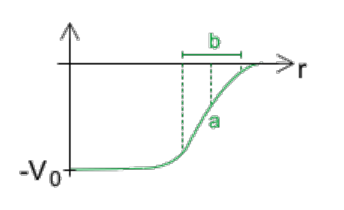
\includegraphics[width=.5\textwidth]{imgs/ep5-fig-4-11.pdf}
\caption{Skizze des Woods-Saxon-Potentials \label{fig:4.11}}
\end{figure}
\begin{align}
\boxed{
V_S(r) = -V_0 \frac{1}{1+e^{\nicefrac{(r-a)}{b}}}
}\\
\sim \text{ Woods-Saxon-Potential}\nonumber
\end{align}
Achtung:
\begin{compactitem}
\item effektives Potential
\item keine zentrale \glqq Kraftquelle\grqq
\item Kräfte \textbf{viel} stärker als in Atom
\end{compactitem}
\item[$\lt$] SG analytisch nicht lösbar
\item[$\lt$] Näherung als harmonischer Oszillator\\
$V_S\lb r\rb  = -V_0 + \frac{1}{2}kr^2, \ r \leq R_k$
\item[$\lt$] In jedem Fall: $V_S\lb  \vec{r}\rb  = V_S(r)$ (sphärisch symmetrisch)
\begin{compactitem}
\item[$\Ra$] Winkelanteil $Y_{lm} (\vartheta, \varphi )$
\item[$\Ra$] Hauptquantenzahl $n$
\item[$\Ra$] $E= \underbrace{E(n,l)}_{2(2l+1)\text{-fach entartet}}$\\
Vorfaktor 2 durch 2 Fermionen pro WF, $2l+1$ Werte für $m$
\end{compactitem}
\begin{align}
\boxed{ E(n,l) = \lb N+\frac{3}{2}\rb  E_0 + \underbrace{\Delta E \lb  n,l\rb }_{=0\text{ für h.O.}}}\\
N=2(n-1)+l\nonumber \\
\Delta E(n,l) = \llb \begin{matrix} \text{klein für kleine } n \text{ und große } l \\ \text{groß für große } n \text{ und kleine } l \end{matrix} \right.
\end{align}
\item[$\Ra$] Baue \glqq Schalen\grqq{} (wie in Atomphysik)
\begin{table}
\centering
\begin{tabular}[!ht]{c|cccc}
$N$ & $nl$ & $2(2l+1)$ & $\sum 2(2l+1)$ & beob?\\
\hline
0 & 1s & 2 &2 & Ja\\
1 & 1p & 6 & 8 & Ja\\
2 & 1d & 10 & 18 & Nein\\
2 & 2s & 2 & 20 & Ja\\
3 & 1f & 14 & 34 & Nein\\
3 & 2p & 6 & 40 & Nein
\end{tabular}
\end{table}
\item[$\ra$] Was fehlt? LS-Kopplung\\
\textbf{Wichtig:} Erfolgt durch \textbf{starke} WW $\Ra$ großer Beitrag zu $V(r)$
\begin{compactitem}
\item[$\lt$] $V_{LS}(r) = \underbrace{\lla V_{LS}\rra}_{<0}\lla \vec{l}\vec{s}\rra$
\item[$\lt$] $\vec{j} = \vec{l} + \vec{s}$ wird bevorzugt maximal\\
$\Ra \ \lla \vec{l}\vec{s}\rra = \frac{1}{2} \lsb  \lla \vec{j}^2\rra - \lla \vec{l}^2\rra - \lla \vec{s}^2 \rra \rsb $\\
$\lla \vec{j}^2\rra = j(j+1)$, $\lla \vec{l}^2\rra = l(l+1)$, $\lla \vec{s}^2\rra = s(s+1)$
\end{compactitem}
\begin{align}
\Ra \ \boxed{ \lla \vec{ls} \rra = \llb \begin{matrix}
\frac{l}{2} \text{ für } j = l+\frac{1}{2}\\
-\frac{l+1}{2} \text{ für } j = l - \frac{1}{2}
\end{matrix} \right. }
\end{align}
\item[$\Ra$] Termschema mit besonders großen Lücken bei
\begin{align*}
\boxed{
\begin{matrix}
 & \text{He} & \text{O} & \text{Ca} & \text{Ni} & \text{Sn} & \text{Pb}\\
 Z = & 2, & 8, & 20, & 28, & 50, &82\\
 N= & 2, & 8, & 20, & 28, & 50, & 82, & 126
\end{matrix}
}
\end{align*}
sogenannte \glqq magische Zahlen\grqq{} $\lt$ Schalen
\item[$\Ra$]  Kerne mit abgeschlossenen Schalen besonders stabil (\glqq magisch\grqq)
\item[$\Ra$] Noch stabiler: \glqq doppelt-magische\grqq{} Kerne:\\
$\boxed{^4_2\text{He}_2, \ ^{16}_8\text{O}_8, \ ^{40}_{20}\text{Ca}_{20}, \ ^{48}_{20}\text{Ca}_{28}, \ ^{208}_{82}\text{Pb}_{126}}$
\item[$\Ra$] Nomenklatur $nL_j$\\ z.B. 2$P_{\nicefrac{3}{2}}$
\item[$\Ra$] Wie in Atomphysik: abgeschlossene Schalen haben Spin, magnetisches Moment $=0$
\item[$\Ra$]  Verhalten von Kernen mit 1 zusätzlichen Nukleon wird durch dieses bestimmt (\glqq Leuchtnukleon\grqq)\\
\textbf{Beispiel:}
\begin{align*}
^{17}_8\text{O}_9, \ Z= 8:\qquad \underbrace{\underbrace{(1S_{\nicefrac{1}{2}})}_2 \underbrace{(1P_{\nicefrac{3}{2}})}_4 \underbrace{(1P_{\nicefrac{1}{2}})}_2}_{\text{abgeschlossen}}\\
N= 9 :\qquad (1S_{\nicefrac{1}{2}})(1P_{\nicefrac{3}{2}})(1P_{\nicefrac{1}{2}}) + (1D_{\nicefrac{5}{2}})\\
\Ra \text{ Spin} \lb  ^{17}_8\text{O}_9\rb  = \underbrace{\text{Spin}\lb  ^{16}_8\text{O}_8\rb }_{=0} + \frac{5}{2}\\
\Ra \text{ magn. Mom.: } \mu\lb  ^{17}_8\text{O}_9\rb  = \mu\lb  ^{16}_8\text{O}_8\rb  + \mu_n  = -1.91\mu_N
\end{align*}
\end{itemize}
